\section{Technische Grundlagen} \label{s:basics}
\begin{comment}
TODO:
- im folgenden bezieht sich Client auf MQTT Client
\end{comment}

Das folgende Kapitel erläutert die erforderlichen technologischen Grundlagen für das tiefere Verständnis des Themas der Thesis.
Das \acs{mqtt} Protokoll wird in Kapitel \ref{s:mqtt} beschrieben.
Kapitel \ref{s:hivemq-broker} handelt von dem HiveMQ Broker und geht insbesondere auf die Cluster Mechanik des Brokers ein.
Abschlie{\ss}end wird die Funktionalität eines Load Balancers am Beispiel von Envoy in Kapitel \ref{s:load-balancing} dargestellt.

\subsection{Message Queuing Telemetry Transport} \label{s:mqtt}
\acf{mqtt} wurde ursprünglich von Doktor Andy Stanford-Clark und Arlen Nipper im Jahr 1999 entworfen, um Gas- und Ölpiplines zu überwachen. Diese lagen oftmals an entlegenen Orten, wie zum Beispiel auf Übersee, und konnten nicht mit Radiowellen oder einem Kabel zum Festland erreicht werden. Zu dieser Zeit war die einzige Option, um Sensordaten auf einen Server zu übertragen, eine auf Datendurchsatz abgerechnete Satellitenkommunikation. Bei mehreren tausend Sensoren wurde somit ein Protokoll benötigt, das die Daten zuverlässig mit minimaler Bandbreite an die Server auf dem Festland übermitteln kann.
\ac{mqtt} wurde im Jahr 2013 von der \ac{oasis} als Open Source standardisiert und wird heutzutage von vielen gro{\ss}en \ac{iot} Plattformen wie AWS IoT und Sparkplug unterstützt.
\cite{WhatMQTTDefinition}\\
Es gibt derzeit zwei Versionen der MQTT Spezifikation: 3.1.1 und 5. Alle Referenzen, falls nicht explizit gekennzeichnet, beziehen sich auf die aktuelle Version 5 des Protokolls.\\
\ac{mqtt} ist ein OSI-Layer 7 \textit{Publish and Subscribe} Protkoll, das auf \acs{tcp} / \acs{ip} aufsetzt. Anders als das Request / Response Paradigma bei \acs{http} ist \ac{mqtt} Event gesteuert und erlaubt Servern eine Nachricht direkt an einen bestimmten Client zu schicken. Somit muss nicht periodisch nach neuen Nachrichten gefragt werden. Zusammen mit einem fixen Paket-Header von nur zwei Byte sorgen diese Eigenschaften für einen geringen Datendurchsatz.\cite{WhatMQTTDefinition}

\subsubsection{Publish and Subscribe} \label{s:publish-subscribe}
\ac{mqtt} nutzt das \textit{Publish and Subscribe} Kommunikationsschema, das eine Struktur bietet, um Nachrichten entkoppelt zwischen Clients auszutauschen. In diesem Schema gibt es zwei unterschiedliche Systeme:
\begin{itemize}
    \item Clients
    \item Broker
\end{itemize}
Clients sind alle Teilnehmer dieses Systems, die Nachrichten empfangen oder veröffentlichen wollen. Um Nachrichten erfolgreich zu vermitteln, wird ein Broker als Mittelsmann verwendet.\cite{teamGettingStartedMQTT}
Jede Nachricht wird durch den Publisher in bestimmte Klassen kategorisiert. Der Publisher wei{\ss} nicht ob, oder wer, an dieser Nachricht interessiert ist und schickt die klassifizierte Nachricht an den Broker.
Clients, die an bestimmten Nachrichten interessiert sind, müssen bei dem Broker eine Subscription erstellen und dabei eine Kategorie angeben.
Somit kann der Broker eingehende kategorisierte Nachrichten an die entsprechenden Clients, auch Subscriber genannt, weiterleiten. Die Kategorie funktioniert wie ein Filter auf alle Nachrichten.
Der Broker kann Nachrichten auch aufbewahren, sodass Clients, die zu einem späteren Zeitpunkt eine Kategorie abonnieren, ebenfalls die vergangenen Nachrichten erhalten.
\cite{EverythingYouNeed}
Durch dieses System entsteht eine Entkopplung der einzelnen Clients auf mehreren Ebenen.
\begin{itemize}
    \item \textbf{Räumliche Entkopplung:} Publisher und Subscriber der Nachricht müssen sich nicht kennen.
      \cite{teamPublishSubscribeMQTT}
    \item \textbf{Zeitliche Entkopplung:} Publisher und Subscriber müssen nicht zur selben Zeit aktiv sein.
      \cite{teamPublishSubscribeMQTT}
    \item \textbf{Synchronisierungs Entkopplung:} Publisher und Subscriber müssen ihre Operationen beim Publizieren und Konsumieren nicht unterbrechen.
      \cite{teamPublishSubscribeMQTT}
\end{itemize}
In verteilten Systemen bietet ein solches Konzept eine einheitliche Abstraktion der Kommunikationsebene.
\cite{domingusDistributedSystemsIntroduction2020}
\begin{figure}
    \centering
    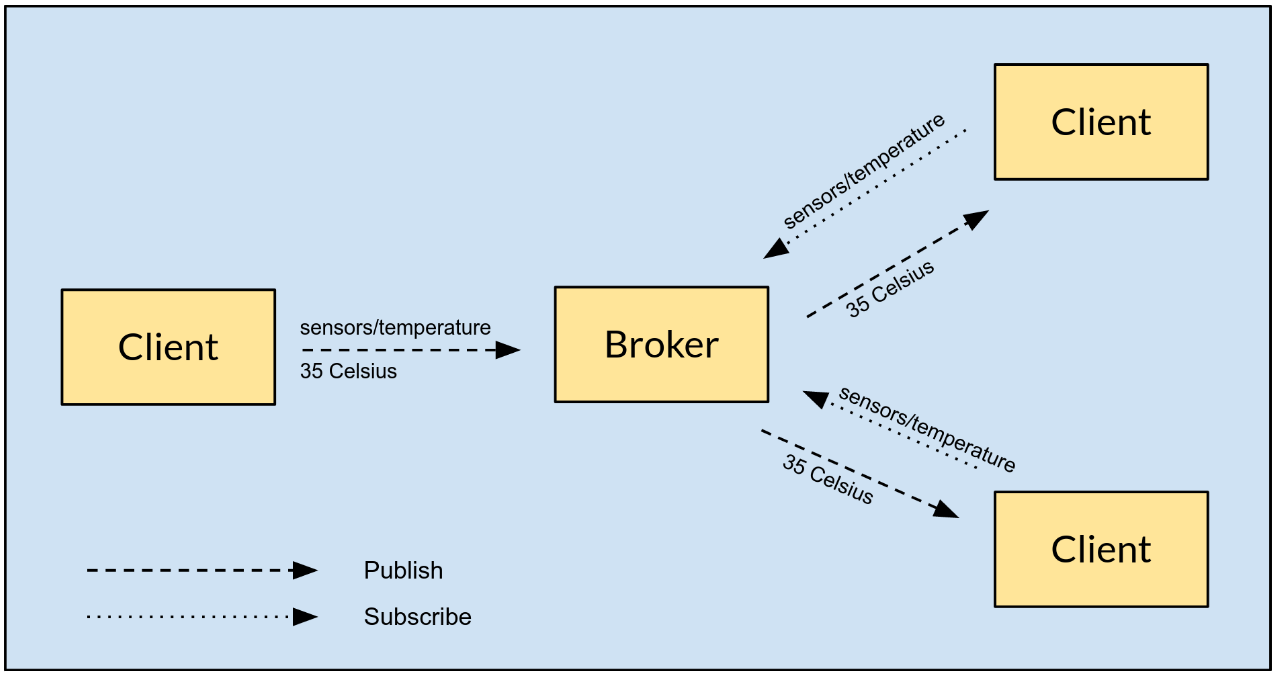
\includegraphics[scale=0.5]{images/publish_subscribe.png}
    \caption{Publish and Subscribe Architektur}
    \label{fig:publish-subscribe}
\end{figure}
\\
Im Kontext \ac{mqtt} werden Nachrichten in ein hierarchisch aufgebautes Topic klassifiziert.
Ein oder mehrere \textit{Topic levels} werden mit einem Schrägstrich (\verb|/|) getrennt und Formen ein Topic. Ein Beispiel für ein Topic mit drei Topic levels ist: \verb|sensors/temperature/celcius|.
Abbildung \ref{fig:publish-subscribe} zeigt einen Client, der auf das Thema \verb|temperature| Nachrichten veröffentlicht. Diese wird an zwei weitere Clients, die das Topic \verb|temperature| abonniert haben, durch den Broker weitergeleitet. Topics müssen auf einem Broker nicht explizit angelegt werden. Sobald ein Client auf einem Topic publiziert oder es abonniert, wird dieses automatisch angelegt.\cite{WhatMQTTDefinition}\\
Beim Abonnieren eines Topics können die Topic levels Wildcards enthalten. Bei Wildcards werden zwischen den folgenden zwei unterschieden:\cite{mqtt5Specification}
\begin{itemize}
    \item Multi-level '\verb|#|': Schlie{\ss}t das Vorgänger- und alle nachfolgenden Topics mit ein.
    \item Single-level '\verb|+|': Schlie{\ss}t alle Topics auf einer einzigen Ebene mit ein.
\end{itemize}
Bei der folgenden Topic-Struktur
\begin{itemize}
    \item \verb|sensors|
    \item \verb|sensors/temperature|
    \item \verb|sensors/temperature/celcius|
    \item \verb|sensors/temperature/kelvin|
    \item \verb|sensors/fuel|
    \item \verb|sensors/fuel/tank1|
    \item \verb|sensors/fuel/tank2|
\end{itemize}
schlie{\ss}t eine Subscription auf \verb|sensors/#| alle Topics mit ein. Bei einem Abonnement auf \verb|sensors/+| sind hingegen nur diese Topics mit eingeschlossen:
\begin{itemize}
    \item \verb|sensors/temperature|
    \item \verb|sensors/fuel|
\end{itemize}

\subsubsection{Quality of Service} \label{s:qos}
Je zuverlässiger eine Nachricht übermittelt werden soll, desto mehr Kommunikationsaufwand verursacht diese Nachricht im gesamten System.
Wenn ein Client wissen will, ob seine Nachricht im Broker eingetroffen ist, muss der Broker dem Client eine entsprechende Rückmeldung liefern. Andernfalls kann der Client seine Nachricht an den Broker schicken ohne eine Rückmeldung zu erwarten. Dies ist im \ac{http} nicht möglicht. Dort muss auf jede Nachricht geantwortet werden.\\
Bei \ac{mqtt} wird die Zuverlässigkeit der Übermittlung einer Nachricht mit einem \textit{\acf{qos}} Level festgelegt. Eine publizierte Nachricht muss einen der drei \ac{qos} Level haben:
\begin{itemize}
    \item \ac{qos} 0: Maximal eine Zustellung der Nachricht.
    \item \ac{qos} 1: Mindestens eine Zustellung der Nachricht.
    \item \ac{qos} 2: Genau eine Zustellung der Nachricht.
\end{itemize}
Bei \ac{qos} Level 1 und 2 werden Handshakes zur Verifizierung der Nachrichtenübermittelung eingesetzt.\cite{mqtt5Specification}

\subsubsection{Retained Message} \label{s:retained-messages}
In \ac{mqtt} kann pro Topic die zuletzt veröffentlichte Nachricht aufbewahrt werden.
Dazu muss im \verb|PUBLISH| Paket die \verb|RETAIN| Kennzeichnung gesetzt werden.
In diesem Fall speichert der Broker die Nachricht mit dem dazugehörigen Topic und \ac{qos} Level ab.
Falls bereits eine aufbewahrte Nachricht (engl. \textit{Retained Message}) auf diesem Topic vorhanden ist, wird sie überschrieben.
Jeder Client, der ein Topic abonniert das eine Retained Message besitzt, bekommt diese Nachricht direkt nach dem Abonnieren zugeschickt.
Dies trifft auch zu, falls das Topic mit der Retained Message durch einen Wildcard Filter abonniert wurde.
\cite{teamRetainedMessagesMQTT}
\\
Um eine Retained Message zu löschen, muss eine neue Nachricht mit der \verb|RETAIN| Kennzeichnung und einem leeren Payload auf dem Topic veröffentlicht werden. Der Broker löscht die aktuelle Retained Message und neue Subscriber werden erst Nachrichten von diesem Topic erhalten, sobald eine neue Nachricht dort veröffentlicht wird.
Wenn ein Topic eine Retained Message (im Folgenden \textit{M1} genannt) aufweist und eine neue Nachricht ohne \verb|RETAIN| Kennzeichnung auf diesem Topic veröffentlicht wird, wird die aktuelle Retained Message M1 nicht überschrieben. Neue Subscriber erhalten weiterhin die Nachricht \textit{M1}.
\cite{mqtt5Specification}
\\
Durch Retained Messages können neue Subscriber direkt einen Wert erhalten, nachdem sie ein Topic abonniert haben. Daher wird eine Retained Messaged auch \textit{last known good value} genannt.
\cite{teamRetainedMessagesMQTT}
\begin{comment}
Als Beispiel dient ein Temperatursensor, der alle zehn Minuten seine Temperatur auf das Topic \verb|sensors/temperature| veröffentlicht. Um den aktuellen Temperaturwert abzufragen gibt es ein Konsolenprogramm, das bei der Ausführung eine Verbindung zu dem Broker herstellt, das Topic \verb|sensors/temperature| abonniert, den ersten erhaltenen Wert auf der Konsole ausgibt, das Topic deabonniert und die Verbindung wieder schlie{\ss}t. Wenn das Programm eine Minute nachdem der Temperatursensor seine Nachricht veröffentlicht hat ausgeführt wird, muss der Benutzer neun Minuten warten bis er die aktuelle Temperatur angezeigt bekommt. Wenn der Temperatursensor seine Nachrichten hingegen als Retained Message veröffentlicht, bekommt das Konsolenprogramm nach dem abonnieren den letzten Temperaturwert und kann diesen anzeigen.
\end{comment}

\subsubsection{Paket Struktur} \label{s:packet-structure}
\ac{mqtt} hat die Absicht ein leichtgewichtiges Protokoll zu sein. Tabelle \ref{table:mqtt-packet-structure} zeigt den Aufbau eines \ac{mqtt} Paketes. Der fixe Header ist zwei Byte gro{\ss} und muss in jedem Paket vorhanden sein. Basierend auf der Art des Paketes, das in dem fixen Header angegeben wird, sind zusätzlich ein variabler Header und weitere Daten möglich.\cite{mqtt5Specification}
\begin{table}[h!]
\centering
\renewcommand{\arraystretch}{1.5}
\begin{tabular}{|c|}
    \hline
    Fixer Header, muss in jedem \ac{mqtt} Paket vorhanden sein \\
    \hline
    Variabler Header, optional \\
    \hline
    Daten des Pakets, optional \\
    \hline
\end{tabular}
\caption{Struktur eines \ac{mqtt} Paketes. Quelle: \cite{mqtt5Specification}}
\label{table:mqtt-packet-structure}
\end{table}
Tabelle \ref{table:fixed-header} zeigt den detaillierten Aufbau des fixen Headers. Im ersten Byte werden Bit sieben bis vier für die spezifische Art des Paketes verwendet. Tabelle \ref{table:mqtt-packet-types} enhält eine Liste mit allen möglichen Pakettypen und deren Wert. Byte zwei gibt die restliche Paketlänge enkodiert als \textit{Variable Byte Integer} an.
\cite{mqtt5Specification}
Die Enkodierung eines \textit{Variable Byte Integer} wird in Kapitel 1.5.5 der \ac{mqtt} 5 Spezifikation \cite{mqtt5Specification} detailliert erklärt.
\begin{table}[h!]
\centering
\renewcommand{\arraystretch}{1.5}
\begin{tabularx}{\textwidth}{|l| *{8}{Y|}}
    \hline
    Bit & 7 & 6 & 5 & 4 & 3 & 2 & 1 & 0 \\
    \hline
    \hline
    Byte 1 & \multicolumn{4}{c|}{\ac{mqtt} Paketart} & \multicolumn{4}{c|}{Paketart spezifische Kennzeichnung} \\
    \hline
    Byte 2 & \multicolumn{8}{c|}{Restliche Paketlänge} \\
    \hline
\end{tabularx}
\caption{Aufbau des fixen \ac{mqtt} Headers. Quelle: \cite{mqtt5Specification}}
\label{table:fixed-header}
\end{table}

\begin{table}[h!]
\centering
\renewcommand{\arraystretch}{1.5}
\begin{tabular}{|l|c|}
    \hline
    \textbf{Name} & \textbf{Wert} \\
    \hline
    \hline
    Reserved & 0 \\
    \hline
    CONNECT & 1 \\
    \hline
    CONNACK & 2 \\
    \hline
    PUBLISH & 3 \\
    \hline
    PUBACK & 4 \\
    \hline
    PUBREC & 5 \\
    \hline
    PUBREL & 6 \\
    \hline
    PUBCOMP & 7 \\
    \hline
    SUBSCRIBE & 8 \\
    \hline
    SUBACK & 9 \\
    \hline
    UNSUBSCRIBE & 10 \\
    \hline
    UNSUBACK & 11 \\
    \hline
    PINGREQ & 12 \\
    \hline
    PINGRESP & 13 \\
    \hline
    DISCONNECT & 14 \\
    \hline
    AUTH & 15 \\
    \hline
\end{tabular}
\caption{Verfügbare \ac{mqtt} Paketarten und deren Wert. Quelle: \cite{mqtt5Specification}}
\label{table:mqtt-packet-types}
\end{table}

\subsubsection{MQTT CONNECT} \label{s:mqtt-connect}
Nachdem eine \ac{tcp} Verbindung zwischen einem Client und einem Broker aufgebaut wurde, muss das erste Paket des Clients ein \verb|CONNECT| Paket sein.
Tabelle \ref{table:mqtt-connect-packet-variable-header} zeigt den Aufbau und Inhalt eines Beispielhaften variablen Headers eines \verb|CONNECT| Paketes.
Die ersten sechs Byte geben den Namen des Protokolls als UTF-8 enkodierten String an. Dieser wird sich in zukünftigen Versionen nicht ändern und dient als Identifikationsmerkmal des \ac{mqtt} Protokolls für Server, die mehrere Protokolle implementiert haben. Byte sieben gibt die verwendete \ac{mqtt} Version des Clients an. In Byte acht kann der Client Kennzeichnungen für die Präsenz der optionalen Daten setzen. Die Länge der Eigenschaften wird mit Byte elf bestimmt. In den Eigenschaften kann der Client zum Beispiel eine maximale Paketgrö{\ss}e oder Themen Aliasse setzen.\cite{mqtt5Specification}\\
Auf den variablen Header folgen die Daten (engl. \textit{Payload}) des \verb|CONNECT| Paketes. Diese sind eine oder mehrere Felder mit ihrer Länge als Präfix. Byte acht des variablen Headers bestimmt das Vorkommen der Felder, die - falls vorhanden - eine strikte Reihenfolge einhalten müssen.
\cite{mqtt5Specification}
\begin{enumerate}
    \item Clientkennung
    \item \textit{Will} Eigenschaften
    \item \textit{Will} Thema
    \item \textit{Will} Payload
    \item Benutzername
    \item Passwort
\end{enumerate}
Die Clientkennung ist als einziges Feld nicht optional. Sie muss ein UTF-8 enkodierter String aus folgenden Zeichen bestehen:
\begin{itemize}
    \item 0-9
    \item a-z
    \item A-Z
\end{itemize}
Eine Clientkennung dient zur Identifikation des aktuellen Zustands des Clients und muss daher einzigartig vergeben sein. Ist bereits ein Client mit der gleichen Kennung mit dem Broker verbunden, wird die Verbindung des existierenden Clients getrennt und es findet ein \textit{Client takeover} statt (siehe \ref{s:client-takeover}).\cite{mqtt5Specification}
\begin{table}[h!]
\centering
\renewcommand{\arraystretch}{1.5}
\begin{tabularx}{\textwidth}{|l|l|c| *{8}{Y|}}
    \hline
    & \textbf{Beschreibung} & \textbf{Wert} &
      \textbf{7} & \textbf{6} & \textbf{5} &
      \textbf{4} & \textbf{3} & \textbf{2} &
      \textbf{1} & \textbf{0} \\
    \hline
    \hline
    Byte 1 & Länge \acs{msb} & 0 & 0 & 0 & 0 & 0 & 0 & 0 & 0 & 0 \\
    \hline
    Byte 2 & Länge \acs{lsb} & 4 & 0 & 0 & 0 & 0 & 0 & 1 & 0 & 0 \\
    \hline
    Byte 3 & UTF-8 Char & 'M' & 0 & 1 & 0 & 0 & 1 & 1 & 0 & 1 \\
    \hline
    Byte 4 & UTF-8 Char & 'Q' & 0 & 1 & 0 & 1 & 0 & 0 & 0 & 1 \\
    \hline
    Byte 5 & UTF-8 Char & 'T' & 0 & 1 & 0 & 1 & 0 & 1 & 0 & 0 \\
    \hline
    Byte 6 & UTF-8 Char & 'T' & 0 & 1 & 0 & 1 & 0 & 1 & 0 & 0 \\
    \hline
    Byte 7 & Protokoll Version & 5 & 0 & 0 & 0 & 0 & 0 & 1 & 0 & 1 \\
    \hline
    Byte 8 &
        \makecell[l]{Benutzername Kennzeichnung \\ Passwort Kennzeichnung \\ \textit{Will} speichern \\ \textit{Will} \ac{qos} Level \\ \textit{Will} Kennzeichnung \\ Frische Session \\ Reserviert} &
        \makecell{1 \\ 1 \\ 0 \\ 01 \\ 1 \\ 1 \\ 0} &
        1 & 1 & 0 & 0 & 1 & 1 & 1 & 0 \\
    \hline
    Byte 9 & Keep Alive \acs{msb} & 0 & 0 & 0 & 0 & 0 & 0 & 0 & 0 & 0 \\
    \hline
    Byte 10 & Keep Alive \acs{lsb} & 10 & 0 & 0 & 0 & 0 & 1 & 0 & 1 & 0 \\
    \hline
    Byte 11 & Länge der Eigenschaften & 0 & 0 & 0 & 0 & 0 & 0 & 0 & 0 & 0 \\
    \hline
\end{tabularx}
\caption{Beispielhaftes \ac{mqtt} CONNECT Paket. Quelle: \cite{mqtt5Specification}}
\label{table:mqtt-connect-packet-variable-header}
\end{table}
Der Broker muss eine \verb|CONNECT| Nachricht von einem Client mit einem \verb|CONNACK| Paket beantworten.\cite{mqtt5Specification}
% TODO länge der eigenschaften kann nicht 0 sein oder ? wegen der clientid

\subsubsection{Last Will Nachricht} \label{s:last-will}
Ein Client kann bei der Verbindung mit einem Broker einen letzten Willen (engl. \textit{Last Will}) als Nachricht definieren. Diese Nachricht wird veröffentlicht, sobald die Verbindung zum Client unterbricht und dieser nicht innerhalb eines definierten Zeitraums seine Verbindung zum Broker wiederaufbauen kann.
Im Fall einer protokollkonformen Terminierung der Verbindung, wird die Last Will Nachricht nicht veröffentlicht.
\cite{soniSURVEYMQTTPROTOCOL}\\
Die Last Will Nachricht kann in sicherheitsrelevanten Applikationen eingesetzt werden, um auf ungeplante Ausfälle von Clients zu reagieren.

\subsubsection{Shared Subscriptions} \label{s:shared-subsriptions}
Mit der fünften Version von \ac{mqtt} wurden \textit{Shared Subscriptions} eingeführt, die das Teilen von Subscriptions unter Clients erlauben. Diese Clients werden in eine \textit{Shared Subscription Group} zusammengefasst. Bei einer normalen Subscription erhält jeder Client, der das gleiche Topic abonniert hat, eine Kopie der Nachricht. Bei einer \textit{Shared Subscription} erhält immer nur ein Client der \textit{Shared Subscription Group} die Nachricht in abwechselnder Reihenfolge. Dieser Mechanismus wird auch als \textit{Client load balancing} bezeichnet, da die Last eines Topics auf mehrere Subscriber verteilt wird.\cite{raschbichlerMQTTHowNew}
Shared Subscriptions verwenden Standard \ac{mqtt} Mechanismen. Jeder Client kann Teil einer Shared Subscription Group werden, indem er folgende Topic Struktur einhält: \verb|$share/GROUPID/TOPIC|.
\begin{itemize}
    \item \verb|$share|: Statische shared Subscription Kennung
    \item \verb|GROUPID|: Identifikation einer Shared Subscription Group. Darf \verb|/|, \verb|#| und \verb|+| nicht enthalten
    \item \verb|TOPIC|: Das zu abonnierende Topic
\end{itemize}
Ein konkretes Beispiel für das abonnieren einer Shared Subscription ist:
\newline
\verb|$share/group1/sensors/temperature|

\newpage

\subsection{HiveMQ Broker} \label{s:hivemq-broker}
Der HiveMQ Broker ist ein Produkt der in 2012 gegründeten Firma HiveMQ \acs{gmbh}. Mit über 130 internationalen Kunden und einem Sitz in Landshut, Deutschland, erleichtert HiveMQ durch ihren \ac{mqtt} Broker die Kommunikation von Geräten und Services untereinander.
\cite{HiveMQCompanya}
\\
Der HiveMQ Broker ist ein auf Java basierter \ac{mqtt} Broker, der auf das Anwendungsfeld \acl{iot} spezialisiert ist. Der Broker unterstützt \ac{mqtt} Version 3 und 5 und ist somit Eclipse Sparkplug kompatibel.
Eclipse Sparkplug ist eine Open Source Spezifikation die ein Framework für \ac{mqtt} Anwendungen bietet, indem sie Definitionen für \ac{mqtt} Topics und \ac{mqtt} Payload Strukturen definiert.
Die Kompatibilität des HiveMQ Brokers mit Sparkplug und die Clusterfähigkeit (siehe Kapitel \ref{s:hivemq-cluster}) ermöglichen den Einsatz des Brokers in Internet of Things Projekten mit mehreren Millionen Clients.
\cite{obermaierMQTTSparkplugEssentials}
\\
Neben dem Anwendungsfeld \ac{iot} kann der HiveMQ Broker auch für \textit{Service to Service} Kommunikation im Backend eigesetzt werden.
Eine Alternative für Event gesteuerte Kommunikation zwischen Services bieten Open Source Broker wie Apache Kafka, RabbitMQ oder ZeroMQ.
\\
Bis 2019 war der Quellcode des HiveMQ Brokers nicht frei zugänglich. Im April 2019 wurde eine \textit{Community Edition} des HiveMQ Brokers unter der Apache 2.0 Lizenz auf GitHub veröffentlicht. Für die Enterprise Edition, mit Features wie Clustering und Control Center, ist eine HiveMQ Lizenz notwendig.

\subsubsection{HiveMQ Cluster} \label{s:hivemq-cluster}
Ein Merkmal des HiveMQ Brokers ist die Möglichkeit ein Broker Cluster zu bilden.
Ein Broker Cluster (folgend Cluster genannt) ist ein verteiltes System, in dem sich mehrere HiveMQ Broker zusammenschlie{\ss}en und eine logische Einheit für Clients bilden.
Demnach macht es für Clients keinen Unterschied, ob sie mit einem einzigen HiveMQ Broker oder mit einem Cluster verbunden sind.
Um dies zu erreichen, tauschen alle Nodes eines Clusters Informationen über Clients und eintreffende Nachrichten aus. Dies geschieht über eine dedizierte Verbindung, die auch Cluster Transport genannt wird.
\cite{HiveMQClusterHiveMQ}
\\
Durch das Zusammenschlie{\ss}en der HiveMQ Broker ensteht eine horizontale Skalierung. Wie in Kapitel \ref{s:domain} bereits erläutert, können sich im Anwendungsfall \ac{iot} mehrere Millionen Clients mit einem \ac{mqtt} Broker verbinden. Hierbei kann eine vertikale Skalierung an ihre Grenzen sto{\ss}en.
\begin{itemize}
    \item \textbf{Vertikale Skalierung:} Fügt mehr Rechen- oder Speichereinheiten zu einem Server hinzu.
      \cite{HowScaleIT}
    \item \textbf{Horizontale Skalierung:} Fügt mehrere Server zu einer logischen Recheneinheit hinzu. Dabei kann die Arbeitslast auf die einzelnen Server verteilt werden.
      \cite{HowScaleIT}
\end{itemize}
Ein HiveMQ Broker in einem HiveMQ Cluster wird als ein HiveMQ Node (im Folgenden Node genannt) bezeichnet.
Damit sich mehrere Nodes zu einem Cluster zusammenschlie{\ss}en muss jeder Node:
\begin{itemize}
    \item ein HiveMQ Enterprise Broker sein.
    \item die anderen Nodes über ein Netzwerk erreichen können.
    \item das \textit{clustering} in seiner Konfiguration eingeschaltet haben.
    \item die anderen Nodes mit der \textit{Cluster Discovery} auffinden können.
\end{itemize}
Die Cluster Discovery beschreibt den Mechanismus wie sich individuelle Nodes gegenseitig finden können, um ein Cluster zu bilden. Es stehen folgende Möglichkeiten zur Verfügung:
\begin{itemize}
    \item \textbf{static:} Jeder Node wird mit einer statischen Liste von allen Nodes und deren \ac{ip} Adresse / Port konfiguriert.
    \item \textbf{multicast:} Nodes finden dynamisch andere Nodes, die dieselbe multicast Adresse und Port benutzen.
    \item \textbf{broadcast:} Nodes finden dynamisch andere Nodes im selben Subnetzwerk, indem sie die Broadcast \ac{ip} Adresse benutzen.
    \item \textbf{extension:} Es kann eine HiveMQ Erweiterung genutzt werden um andere Nodes zu entdecken.
\end{itemize}
HiveMQ ist in der Lage die Clustergrö{\ss}e zur Laufzeit dynamisch anzupassen. Diesen Mechanismus muss der gewählte Cluster Discovery Modus unterstützten.
\cite{HiveMQClusterHiveMQ}

\subsubsubsection{Überlastschutz} \label{sb:overload-protection}
HiveMQ stellt einen eingebauten Überlastschutz (engl. \textit{Overload Protection}) für ein HiveMQ Cluster bereit. Jeder Node eines Clusters ist in der Lage die Rate der eingehenden Nachrichten zu reduzieren. Dieser Mechanismus erhöht die Stabilität des Clusters, indem gezielt Clients, die zu einer Überlast beitragen, gedrosselt werden.
\cite{ClusterOverloadProtection}
Dadurch kann sich das Cluster von einer Überlastsituation erholen, ohne die Service Qualität für Clients, die nicht der Überlastsituation beitragen, zu beeinträchtigen.
Jeder Node eines Clusters berechnet durchgehend einen individuellen \textit{Overload Protection Level} auf Basis der Menge aller:
\begin{itemize}
    \item eingehenden \verb|PUBLISH| Nachrichten
    \item Retained Messages
    \item verbundenen Clients
    \item Queued Messages
\end{itemize}
Das Drosseln von Clients basiert auf einem Credit System. Jeder Client erhält nach dem Aufbau einer Verbindung ein Guthaben von 50,000 Credits.
Für jede Veröffentlichung einer Nachricht werden die Credits des Clients reduziert.
Diese werden alle 200 Millisekunden um einen bestimmten Wert regeneriert, bis das maximale Guthaben von 50,000 erreicht wurde. Der Regenerationswert richtet sich nach dem derzeitigen Overload Protection Level des Nodes, mit dem der Client verbunden ist.
\cite{ClusterOverloadProtection}
\\
Hat ein Client alle seine Credits verbraucht, wird \ac{tcp} Backpressure auf dem Socket des Clients angewandt woraufhin dieser keine Nachrichten mehr veröffentlichen kann.
Überschreitet der Zeitraum, in dem \ac{tcp} Backpressure für einen Client angewandt wird, den konfigurierten Keep-Alive Wert der Verbindung, wird diese unterbrochen.
Ist der Zeitraum, in dem \ac{tcp} Backpressure für einen Client angewandt wird, länger als der konfigurierte Keep-Alive Wert, wird die Verbindung des Clients unterbrochen.
Neben \ac{mqtt} Clients kann auch eine Topologieänderung des Clusters zu einer Erhöhung des Overload Protection Levels führen.
\cite{ClusterOverloadProtection}

\subsubsection{Persistente Session} \label{s:persistent-session}
Um Nachrichten von einem \ac{mqtt} Broker zu erhalten, muss sich ein Client mit diesem verbinden und eine Subscription auf einem Topic erstellen. Alle Subscriptions die ein Client erstellt, werde mit der \ac{tcp} Verbindung des Clients assoziiert.
Jedes Mal, wenn die Verbindung zum Client unterbrochen wird, muss die Verbindung erneut aufgebaut und alle Subscriptions erneut erstellt werden.
Für einen Client mit limitierten Ressourcen ist dies eine Belastung.
Um diese Belastung zu reduzieren, kann der Client beim Aufbau der Verbindung eine persistente Session anfordern, indem das entsprechende Bit eins von Byte acht des variablen Headers der \verb|CONNECT| Nachricht (siehe Tabelle \ref{table:mqtt-connect-packet-variable-header}) auf null setzt.
Ist dieses Bit hingegen auf eins gesetzt, werden alle Nachrichten und Informationen von vorherigen Sessions gelöscht.
Eine persistente Session speichert folgende Daten auf dem Broker:
\begin{itemize}
    \item Die Existenz einer persistenten Session. Als Identifikation wird die Clientkennung verwendet.
    \item Alle Subscriptions des Clients.
    \item Alle Nachrichten mit einem \ac{qos} Level eins oder zwei, die der Client noch nicht bestätigt hat.
    \item Alle Nachrichten mit einem \ac{qos} Level eins oder zwei, die der Client aufgrund der unterbrochenen Verbindung nicht erhalten konnte.
    \item Alle Nachrichten mit einem \ac{qos} Level zwei, die der Client veröffentlicht hat und noch nicht bestätigt wurden.
\end{itemize}
Bei einer persistenten Session muss neben dem Broker auch der Client Informationen speichern. Er ist verantwortlich die folgenden Daten zu persistieren:
\begin{itemize}
    \item Seine eigene Clientkennung. Diese wird als Identifikationsmerkmal einer persistenten Session auf dem Broker genutzt und muss bei einer erneuten Verbindung immer gleich sein.
    \item Alle \ac{qos} Level eins oder zwei Nachrichten, die noch nicht vom Broker bestätigt wurden.
    \item Alle \ac{qos} Level zwei Nachrichten, die der Client vom Broker erhalten hat und noch nicht vollständig bestätigt wurden.
\end{itemize}
Sobald ein Client die Verbindung zu einem Broker verliert und eine persistente Session aktiv ist, versucht der Broker die Daten des Clients solange wie möglich zu persistieren, bis dieser sich erneut verbindet. Falls der Broker während der Zeit, die der Client nicht verbunden ist, keinen verfügbaren Ressourcen mehr hat, besteht die Möglichkeit, dass die persistente Session vom Broker gelöscht wird.
\cite{teamPersistentSessionQueuing}

\subsubsubsection{Client Takeover} \label{s:client-takeover}
Wie bereits im Kapitel \ref{s:persistent-session} beschrieben kann ein Client eine persistente Session bei einem Broker anfordern. Dabei werden zum Beispiel Nachrichten mit einem \ac{qos} Level von eins oder zwei auf dem Broker nachgehalten, falls der Client seine Verbindung verliert. Ein Client Takeover findet statt, wenn der Broker eine neue Client Verbindung erhält aber noch eine offene Verbindung mit derselben \ac{clientid} hat. Dies kann bei \textit{halb-offenen \acs{tcp} Verbindungen} vorkommen, die, wie Andy Stanford-Clark beschreibt, bei \ac{tcp} auftreten können:\newline
``Although TCP/IP in theory notifies you when a socket breaks, in practice, particularly on things like mobile and satellite links, which often 'fake' TCP over the air and put headers back on at each end, it’s quite possible for a TCP session to 'black hole', i.e. it appears to be open still, but in fact is just dumping anything you write to it onto the floor.''\cite{WhyKeepaliveNeeded}\newline
Der Broker beendet die existierende Verbindung und assoziiert die persistente Session - falls vorhanden - nun mit dem neuen Client.
\cite{teamKeepAliveClient}
\newpage

\subsection{Load Balancing} \label{s:load-balancing}
Load balancing wurde um 1990 als Unterstützung für horizontale Skalierung eingeführt, um Traffic auf Server-Infrastrukturen zu verteilen. Dadurch sollte eine erhöhte Verfügbarkeit der Services für Endnutzer erzielt werden.
\cite{LoadBalancing101}
Bei einer horizontalen Skalierung werden nicht die Ressourcen eines einzelnen Servers erweitert, wie bei der vertikalen Skalierung, sondern weitere Server bereitgestellt. Es gibt mehrere Gründe wann eine vertikale Skalierung an ihre Grenzen stö{\ss}t:
\begin{itemize}
    \item Der Server ist nicht mehr erweiterbar an \acs{cpu}, \acs{ram} oder Speicherplatz.
    \item Ein neustarten des Servers um eine vertikale Skalierung durchzuführen ist nicht möglich.
    \item Es muss eine Hochverfügbarkeit erzielt werden.
\end{itemize}
\cite{bourkeServerLoadBalancing2001}
Ein \acl{lb} wird bei der horizontalen Skalierung den einzelnen Servern vorgeschaltet, um einkommenden Traffic basierend diverser load balancing Algorithmen an die entsprechenden Server zu verteilen.
Je nach Algorithmus sorgt der \ac{lb} dadurch für ein gleimä{\ss}ges verteilen der Last auf das gesamte System. Es ist ebenfalls möglich ausgefallene Server zu detektieren und die Last auf verbleibende Server umzuleiten.
\\
Load balancing kann Software- und Hardwareseitig betrieben werden. Als Hardware \ac{lb} wird oftmals ein OSI-Layer vier oder sieben Switch verwendet. Dabei müssen alle Server, die Last erhalten sollen, direkt an den Hardware \ac{lb} angeschlossen werden.
\cite{WasIstLoad2016}
Software load balancing braucht, anders als Hardware load balancing, keine dedizierte Hardware und kann in jedem Server, Container oder jeder virtuellen Maschine eingesetzt werden.
\cite{SoftwareLoadBalancing}
Dabei kann jegliche Funktionalität eines \acp{hlb} vollständig ersetzt und erweitert werden. Software load balancing bietet mehr flexibilität gegenüber Hardware load balancing auf Kosten von Performance.
\cite{WhatLoadBalancer}
\\
Load balancing kann zwischen Layer vier bis sieben des \ac{osi}-Modells stattfinden.
\cite{WhatLoadBalancer}
Das \ac{osi}-Modell standardisiert die Kommunikation zwischen verschiedenen Computer Systemen in sieben Layern.
\begin{enumerate}
    \item Bitübertragungsschicht (engl. \textit{Physical Layer})
    \item Sicherrungsschicht (engl. \textit{Datalink Layer})
    \item Vermittlungsschicht (engl. \textit{Network Layer})
    \item Transportschicht (engl. \textit{Transport Layer})
    \item Sitzungsschicht (engl. \textit{Session Layer})
    \item Darstellungsschicht (engl. \textit{Presentation Layer})
    \item Anwendungsschicht (engl. \textit{Application Layer})
\end{enumerate}
\cite{WhatOSIModel}
\paragraph{Layer 4 Load Balancing}
Der \ac{lb} lenkt den Traffic basierend von Infromationen des Network und Transport Layers. Darunter befinden sich \ac{tcp} und \ac{udp} Ports der Pakete sowieso Empfänger und Absender \ac{ip} Adressen. Layer vier \ac{lb} inspizieren für die Weiterleitung nicht die Daten des Paketes.
\cite{WhatLoadBalancer}

\paragraph{Layer 7 Load Balancing}
Ein Layer sieben \ac{lb} inspiziert die Daten des gesendeten Paketes. Dafür muss der \ac{lb} in der Lage sein das verwendetet Protokoll zu parsen. Es können komplexere Weiterleitungregeln als bei einen Layer vier \ac{lb} implementiert werden. Bei \ac{http} können beispielsweise Weiterleitungsentscheidungen basierend des \ac{http} Headers oder des \ac{http} Pfades getroffen werden.
\cite{WhatLoadBalancer}
\\
In verteilten System, zum Beispiel einem HiveMQ Cluster, bieten \acl{lb} eine transparente Abstraktion für Clients. Der Client verbindet sich mit einem \ac{lb} und wird an einen HiveMQ Node weitergeleitet ohne die Server-Infrakstruktur des HiveMQ Clusters zu kennen. Für den Client macht es den Anschein, als würde der \ac{lb} eine einziger HiveMQ Broker sein, der seinen Service anbietet.

\subsubsection{Load Balancing Algorithmen} \label{sb:lb-algo}
Der \acl{lb} bestimmt anhand eines load balancing Algorithmus an welchen Server eine neue Anfrage verteilt wird.
Welcher Algorithmus verwendet wird, hängt von dem Einsatz des Load Balancers ab.
Das Protokoll, die Server-Infrakstruktur oder das Verhalten der Clients sind wichtige Faktoren für die Auswahl des Algorithmus.
\\
Folgend werden die weit verbreitesten load balancing Algorithmen erläutert.

\paragraph{Round Robin}
Alle Server werden in eine Liste eingetragen. Der Round robin Algorithmus leitet Traffic immer an den ersten Server in der Liste weiter und verschiebt diesen Server danach an das Ende der Liste.
Dieser Algorithmus teilt alle Anfragen gleichmä{\ss}ig auf die Server auf und findet oft Anwendung wenn alle Server die gleichen Ressourcen zur verfügung haben.
\cite{WhatLoadBalancer}

\paragraph{Least Connection}
Der least connection Algorithmus hält alle aktiven Client Verbindungen pro Server nach und verteilt neue Anfragen immer an den Server, der die wenigsten aktiven Verbindungen hat.
\cite{WhatLoadBalancer}

\paragraph{Consistent Hashing}
Der \ac{lb} bestimmt den Server anhand eines Hash-Wertes von diversen Daten des eintreffenden Paketes vom Client.
Mögliche Daten sind Quell-, Ziel \ac{ip} Adresse, Port oder Domain Name. Durch diesen Algorithmus werden wiederkehrende Clients mit den selben Hash-Werten immer mit dem selben Server verbunden.
\cite{WhatLoadBalancer}

\subsubsection{Envoy} \label{s:envoy}
Envoy ist ein \ac{osi}-Layer sieben Proxy und für gro{\ss}e moderne Service orientierte Architekturen von Lyft entwickelt worden.
Im September 2017 wurde Envoy an die \textit{Cloud Native Computing Foundation} gestiftet, die Cloud Projekte wie Kubernetes, Prometheus, containerd und Jaeger verwaltet.
Der Envoy Quellcode wird öffentlich auf GitHub versioniert und hat stand April 2021 bereits 670 Kontributoren und 16.500 Sterne auf GitHub gesammelt. \cite{EnvoyproxyEnvoy2021}
\\
Der in C++ programmierte und hoch performante \ac{lb} Envoy stellt folgende abstrakte Features bereit:
\begin{itemize}
    \item \textbf{\acs{osi}-Layer 3/4 Filter:} Envoy erlaubt das Dazuschalten von \acs{tcp} oder \acs{udp} Filtern in die Netzwerk Pipeline. Filter wie zum Beispiel für MongoDB, Redis, \ac{tls} Authentifizierung wurden bereits in Envoy implementiert. Benutzerdefinierte Filter können direkt in C++ implementiert und eingebunden oder als \ac{wasm} Modul integriert werden.
      \cite{WhatEnvoyEnvoy}
    \item \textbf{\acs{http} \ac{osi}-Layer 7 Filter:} Aufgrund der Popularität von \ac{http} wurden diverse \ac{osi}-Layer 7 \ac{http} Filter in Envoy implementiert. Filter wie \textit{buffering}, \textit{routing} und \textit{rate-limiting} sind bereits in Envoy integriert und können über einen \ac{http} Connection Manager konfiguriert werden.
      \cite{WhatEnvoyEnvoy}
    \item \textbf{Dynamische Konfiguration:} Envoy kann dynamisch über eine \textit{Data-Plane API} provisioniert werden. Dabei können Daten wie Cluster, \ac{http} Routen, Listener Sockets oder \ac{tls} Zertifikate dynamisch von einer externen Quelle bereitgestellt werden.
      \cite{WhatEnvoyEnvoy}
    \item \textbf{Observeability:} Envoy verfolgt das Ziel transparete Netzwerke zu erschaffen. Um dies zu erreichen werden umfangreiche Statistiken bereitgestellt, die zum Beispiel mit \textit{statsd} aggregiert werden können.
      \cite{WhatEnvoyEnvoy}
\end{itemize}
Envoy wird unteranderem bei Slack \cite{MigratingMillionsConcurrent2021} als \acl{lb} für Websockets eingesetzt. Zudem findet Envoy Anwendung in \textit{service-meshes} als Edge Proxy bei Istio \cite{Istio} und Google Traffic Director \cite{TrafficDirectorGoogle}.

\begin{comment}
\subsubsubsection{Architecture}
test
\cite{datawireEnvoyInternalsDeep2018}

warum envoy?
- programmierbar vs konfigurierbar -> envoy ist eher programmierbar -> vor allem durch wasm
- envoy teil: warum habe ich envoy gewählt -> ein paar zeilen
  - control plane, pipeline, eigenschaften, hot reload, warum nimmt man envoy
\end{comment}
\newpage
